\begin{mainquestion}{singlefreqgain}{Complex Gain at a Single Frequency}

A black box with an input and output is found to have a voltage gain magnitude $\left|H\left(j\omega_{0}\right)\right| = 17$ at a frequency $\omega_{0}$, with $v_{o}(t)$ leading $v_{i}(t)$ by $17^{\circ}$ (both voltages are assumed to be sinusoids).

\begin{partquestion}{complexforms}{Express the gain at $\omega_{0}$ as a complex number in both Cartesian and Euler forms. Be careful with your degrees and radians!}
\begin{answer}
The problem describes a voltage gain $H(j\omega)$ at a specific frequency $\omega_{0}$:

\[
H\left(j\omega_{0}\right) = 17e^{j2\pi\left(\frac{17}{360}\right)} = 17e^{j(0.297)}
\]

In Cartesian form, it becomes:

\begin{align*}
H\left(j\omega_{0}\right) &= 17\cos\left(0.297\right)+j17\sin\left(0.297\right)\\
&= 16.26+4.97j
\end{align*}

\end{answer}
\end{partquestion}

\begin{partquestion}{outputwaveform}{Find an expression for $v_{o}(t)$ at $\omega_{0}$ assuming $v_{i}(t) = \cos\left(\omega_{0}t - 17^{\circ}\right)$. Sketch both input and output waveforms vs. time, on the same set of axes.}
\begin{answer}
Using Euler's notation, we have:

\[
\mathbf{V_{\it{i}}} = e^{j\left(\omega_{0}t - 2\pi\left(\frac{17}{360}\right)\right)}
\]

so
\begin{align*}
\mathbf{V_{\it{o}}} &= \mathbf{V_{\it{i}}}H\left(j\omega\right)\\
&=17e^{j\left(\omega_{0}t + 2\pi\left(-\frac{17}{360}+\frac{17}{360}\right)\right)}\\
&=17e^{j\omega_{0}t}
\end{align*}

This implies that $v_{o}(t) = 17\cos\left(\omega_{0}t\right)$.

\begin{center}
    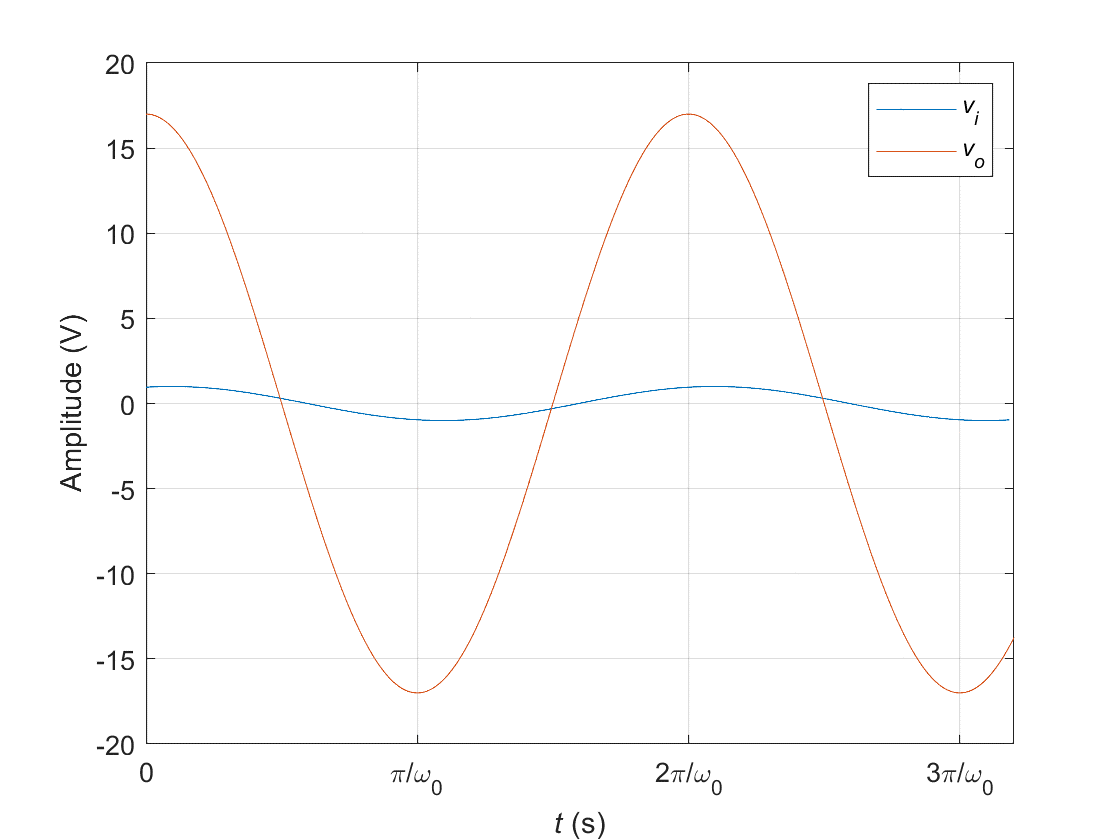
\includegraphics[width=5.2in]{questionbank/networks/single_frequency_gain/v0/waveforms.png}
\end{center}
\end{answer}
\end{partquestion}

\begin{partquestion}{otherfrequencies}{What can we say about the gain at $2\omega_{0}$? What about $\frac{1}{2}\omega_{0}$?}
\begin{answer}
Absolutely nothing, for either! We are only given information about the gain at one frequency, namely $\omega_{0}$. It is entirely unspecified for any other frequency of consideration.
\end{answer}
\end{partquestion}

\end{mainquestion}